\section{Analysis}
\FloatBarrier % Now figures cannot float above section title

\subsection*{a}
Using the data in Table 2, the force vs deformation plot can be derived as \autoref{f3}. Also, from the lecture in week 7, we can learn that the total bending moment diagram is as follows


\begin{figure}[htbp]
    \centering
    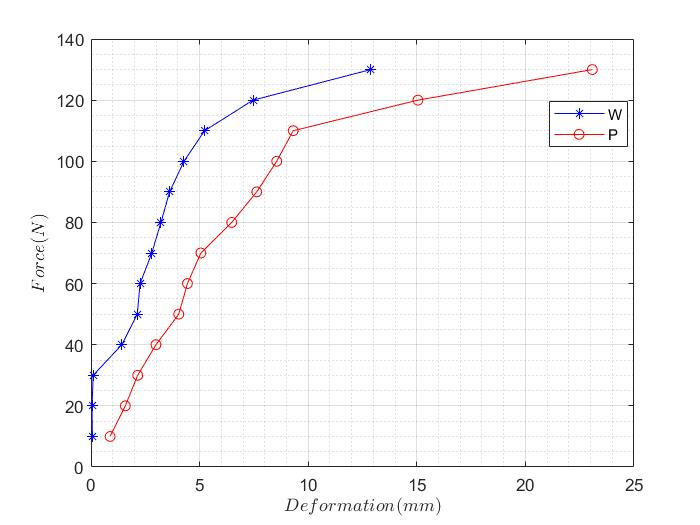
\includegraphics[width=9cm]{./fig/17.jpg}
    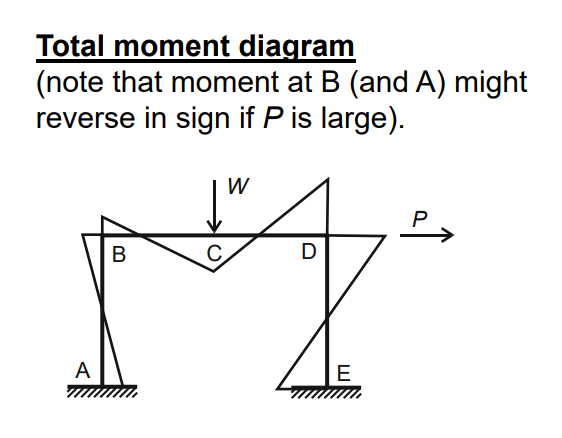
\includegraphics[width=7cm]{./fig/16.png}
    \caption{Force vs deformation and total moment diagram}
    \label{f4}
\end{figure}


The chart illustrates the relationship between the strength and deformation of steel, which can be discussed in two different situation.

$\bullet$ W<110N,P<110N: Elastic deformation: The relationship between the elastic deformation variable and the external force is linear.

$\bullet$ W$\geq$110N,P$\geq$110N: Plastic deformation: The relationship between force and deformation is nonlinear, i.e., the strain shows a rapid increase with the increase of stress.

From the total moment diagram (\autoref{f3}), it can be seen that the bending moment at point D is the largest, and this point will be the first point in the experiment to achieve plastic deformation.

In \autoref{f2}, The P-W graph is piecewise and if the combination of the P and W exceeds the closed figure on the left, The collapse will happen. In this case$(y=x)$, the collapse load for the frame was $W=148.63N,P=148.63N$.

\textit{Can you identify at which load each plastic hinge formed?}


\subsection*{b}

\begin{figure}[htbp]
    \centering
    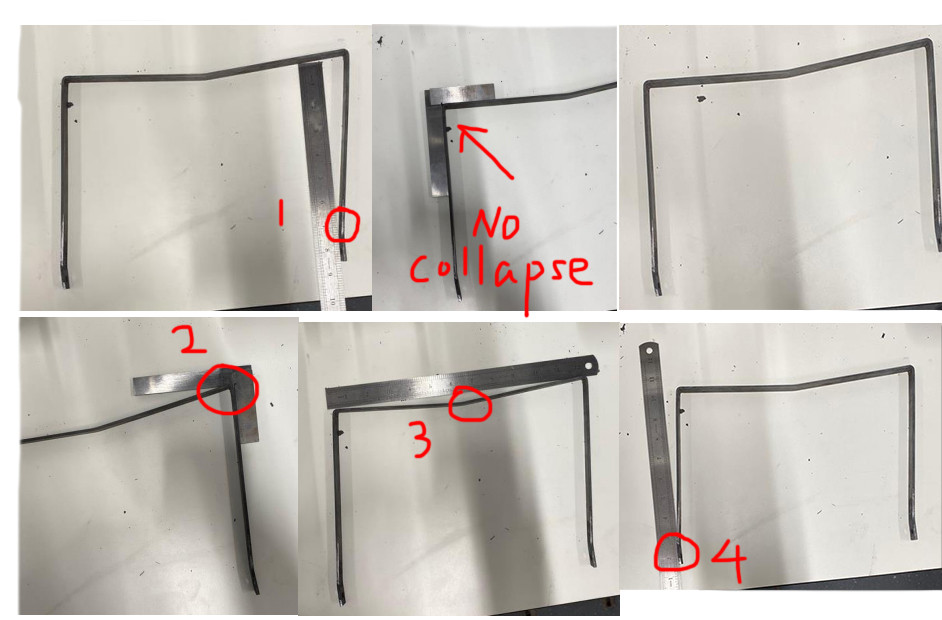
\includegraphics[width=10cm]{./fig/18.jpg}
    \caption{Experimental results}
    \label{f5}
\end{figure}

There are 4 plastic hinges at the moment of the collapse of the frame. Compare \autoref{f2} and \autoref{f5} we can find: 

$\bullet$ After the force load, the upper left corner of the frame did not rotate, and the angle between the beam and column was still degrees.

$\bullet$ The angle of rotation of the plastic collapse occurring at points 1,4 is $\theta$(in \autoref{f2}).

$\bullet$ The angle of rotation of the plastic collapse occurring at points 2,3 is $2\theta$(in \autoref{f2}).

\subsection*{c}
\subsubsection*{i}

The theoretical plastic collapse load derived from Section 2 is 148.63N, while the actual collapse load is in the region of 110N.

The comparison leads to the conclusion that the actual collapse load will be less than the theoretical value for these possible reasons:

$\bullet$ Material inhomogeneity: there are microscopic defects, grain boundaries, organisation and other factors in the actual material, which can lead to differences in the mechanical properties of the material, thus affecting the plastic deformation and strength of the material.

$\bullet$ Differences in test conditions: The plastic collapse load of a material often needs to be determined experimentally, and differences in experimental conditions (e.g. temperature and humidity) can also affect the difference between the actual plastic collapse load and the theoretical value.

\subsubsection*{ii}

\subsubsection*{iii}